%
%
%RELAÇÃO DE COMANDOS LaTeX úteis:
%
%
%
%Como adicionar uma abreviatura na lista:
\abbrev{Abbreviation}{Abbreviation Definition}

%Como adicionar um símbolo na lista:
\symbl{Symbol}{Symbol Definition}

%Adicionar nota de rodapé:
\footnote{Este é um teste para checar o correto funcionamento das notas de rodapé.}

%Subníveis textuais a serem empregados:
%Nível 1
\chapter{}

%Nível 1.1
\section{}

%Nível 1.1.1
\subsection{}

%Nível 1.1.1.1
\subsubsection{}
\addtocounter{secnumdepth}{1}

%Esse aqui posso até usar, porém sem ser numerado mesmo, e do jeito que está, i.e. como parágrafo mesmo, sem alterar o comportamento padrão da estrutura.
%Nível 1.1.1.1.1
\paragraph{}

%Esse aqui não será usado, seguindo o padrão prescrito na norma brasileira.
%Nível 1.1.1.1.1.1
\subparagraph{}

%Como incluir ilustrações
\begin{grafico}[!hbt]
  \centering
  \caption{Um gráfico de exemplo}
  \makebox[0pt]{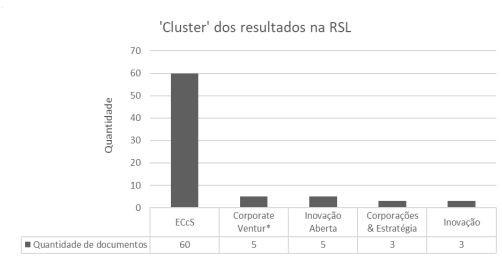
\includegraphics[]{Gráficos/grafico-exemplo}}
  \source{Elaborado pelo autor}
  \label{grafico-exemplo}
\end{grafico}

%ENVIRONMENTS MAIS COMUNS
\begin{itemize}
  \item
\end{itemize}

\begin{enumerate}
  \item
\end{enumerate}

\begin{description}
  \item[]
\end{description}

- tabbing
- bibliography
\=
\\
\>

\includegraphics[aopt]{}

%Como citar?
\cite{ckey}

%Aparece na lista de referências sem ser citada
\nocite{*}
